\documentclass[a4paper,12pt]{article}

% --- Packages ---
\usepackage{fontspec}
\usepackage[vietnamese,english]{babel}
\usepackage{fancyhdr}
\usepackage{extramarks}
\usepackage{amsmath, amsthm, amsfonts}
\usepackage{tikz}
\usepackage[plain]{algorithm}
\usepackage{algpseudocode}
\usepackage{setspace}
\usepackage{graphicx}
\usepackage{geometry}

\begin{document}


\section{Phân phối Đều (Uniform Distribution)}

\textbf{Phân phối đều} là một trong những phân phối xác suất cơ bản nhất, đặc trưng bởi \textbf{xác suất hoặc mật độ phân bố đều trên toàn bộ miền xác định}.  
Phân phối đều có hai loại:
\begin{itemize}
    \item \textbf{Phân phối đều rời rạc (Discrete Uniform Distribution)}.
    \item \textbf{Phân phối đều liên tục (Continuous Uniform Distribution)}.
\end{itemize}

Ta ký hiệu:
\[
X \sim \mathrm{Uniform}(a, b), \quad -\infty < a < b < +\infty
\]

\subsection{Phân phối Đều Rời Rạc}

\subsubsection{Probability Mass Function - PMF}:

Hàm trọng lượng xác suất của phân phối Đều là:
Giả sử biến ngẫu nhiên \( X \) có phân phối đều rời rạc trên tập \( \{x_1, x_2, \ldots, x_n\} \). Khi đó:

\[
P(X = x) =
\begin{cases}
\displaystyle \frac{1}{n}, & x \in \mathcal{S}, \\[1em]
0, & \text{ngược lại}.
\end{cases}
\]

hay viết ngắn gọn:
\[
\mathrm{PMF}(x) = \frac{1}{n}, \quad \forall x \in \{x_1, x_2, \ldots, x_n\}.
\]

\subsubsection{Cumulative Distribution Function - CDF}

Hàm xác suất tích lũy được định nghĩa là:
\[
F(x) = P(X \le x) =
\begin{cases}
0, & x < x_1 \\[0.5em]
\dfrac{\text{số phần tử } \le x}{n}, & x_1 \le x \le x_n \\[0.8em]
1, & x \ge x_n
\end{cases}
\]
  
\begin{figure}[h!]
    \centering
    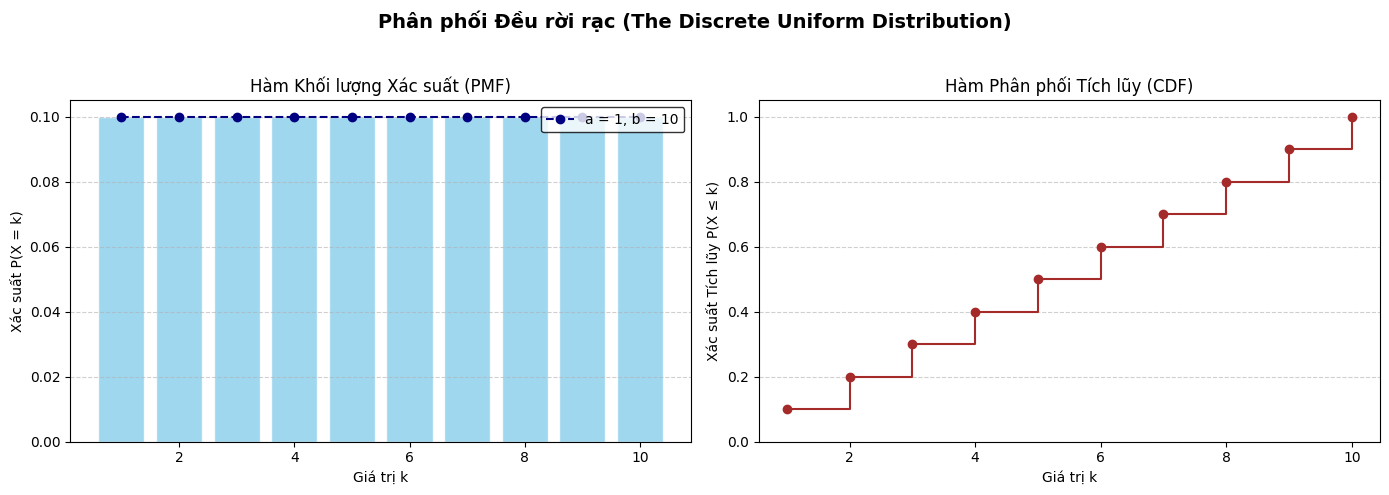
\includegraphics[width=0.8\textwidth]{images/Uniform_PMF_and_CDF.png}
    \caption{Biểu đồ Hàm Khối lượng Xác suất (PMF) và Hàm Phân phối Tích lũy (CDF) của Phân phối Đều Rời Rạc.}
    \label{fig:uniform_disc_dist}
\end{figure}

\subsection{Phân phối Đều Liên Tục}
\subsubsection{Probability Density Function - PDF}:
Hàm mật độ xác suất của phân phối đều liên tục được định nghĩa như sau:  
Giả sử biến ngẫu nhiên \( X \) có phân phối đều liên tục trên đoạn \([a, b]\). Khi đó:

\[
f(x; a, b) =
\begin{cases}
\displaystyle \frac{1}{b - a}, & a \le x \le b, \\[1em]
0, & \text{ngược lại}.
\end{cases}
\]

Điều này phản ánh rằng mọi giá trị trong khoảng \([a, b]\) đều có \textbf{mật độ xác suất như nhau}.


\subsubsection{Cumulative Distribution Function - CDF}

Hàm phân phối tích lũy (CDF) của phân phối đều liên tục được xác định bằng cách tích phân hàm mật độ:

\[
F(x; a, b) = P(X \le x) = \int_{-\infty}^x f(t; a, b)\, dt.
\]

Do đó:

\[
F(x; a, b) =
\begin{cases}
0, & x < a, \\[0.8em]
\dfrac{x - a}{b - a}, & a \le x \le b, \\[1em]
1, & x > b.
\end{cases}
\]

  
\begin{figure}[h!]
    \centering
    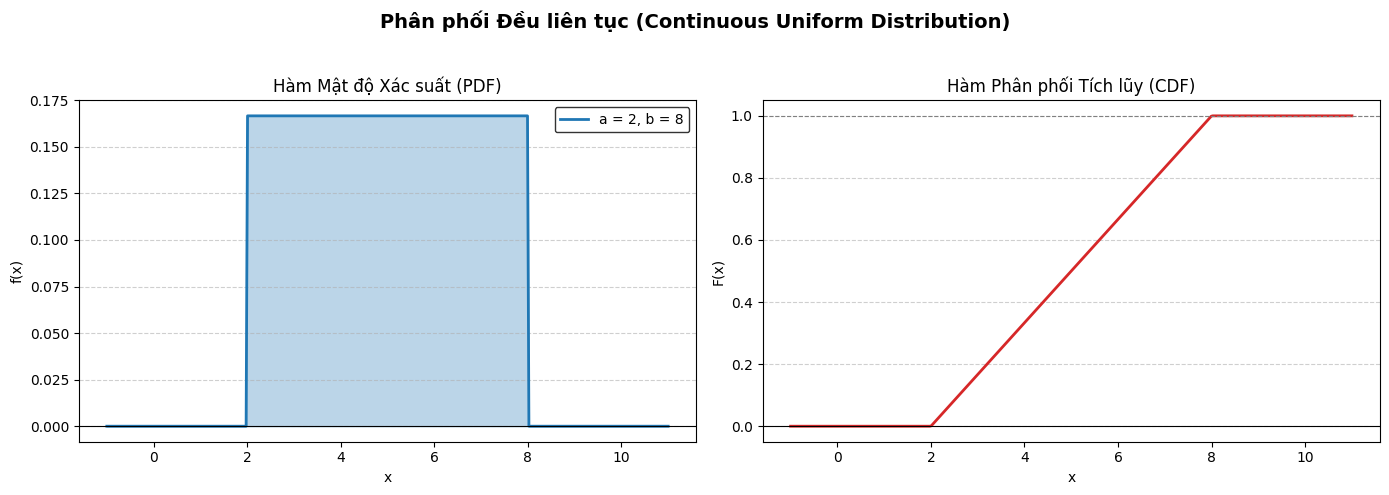
\includegraphics[width=0.8\textwidth]{images/Uniform_PDF_and_CDF.png}
    \caption{Biểu đồ Hàm Mật độ Xác suất (PDF) và Hàm Phân phối Tích lũy (CDF) của Phân phối Đều Liên tục.}
    \label{fig:uniform_cont_dist}
\end{figure}

\subsubsection{Các đặc trưng thống kê}

\begin{itemize}
    \item \textbf{Kỳ vọng (Mean):}
    \[
    \mathbb{E}[X] = \frac{a + b}{2}
    \]
    \item \textbf{Phương sai (Variance):}
    \[
    \mathrm{Var}(X) = \frac{(b - a)^2}{12}
    \]
    \item \textbf{Mode:} Mọi giá trị trong $[a, b]$ đều có cùng mật độ nên không có mode duy nhất.
    \item \textbf{Median:}
    \[
    \mathrm{Median}(X) = \frac{a + b}{2}
    \]
    \item \textbf{Miền xác định:}
    \[
    x \in [a, b]
    \]
\end{itemize}

\subsubsection{Tính chất hình dạng (Shape)}

\begin{itemize}
    \item Phân phối đều liên tục có \textbf{dạng hình chữ nhật}, vì mật độ xác suất không đổi trong $[a, b]$.
    \item Phân phối này \textbf{đối xứng hoàn toàn} quanh trung điểm $\frac{a + b}{2}$.
    \item Không có độ lệch (skewness = 0) và hệ số nhọn (kurtosis excess = $-1.2$).
\end{itemize}

\subsubsection{Ví dụ dữ liệu và ứng dụng thực tế}

\paragraph{Ứng dụng 1: Kiểm soát chất lượng sản phẩm trong dây chuyền sản xuất.} 
Trong nhiều quy trình sản xuất, các sai số gia công cơ khí (như độ lệch kích thước, độ sâu mũi khoan, hoặc vị trí khoan lỗ) thường nằm trong một khoảng xác định \([a, b]\). Khi không có yếu tố nào khiến sai số tập trung về phía nào trong khoảng, một giả định hợp lý là sai số này tuân theo phân phối đều liên tục \(\mathcal{U}(a, b)\). 
Mô hình này giúp các kỹ sư chất lượng ước lượng xác suất sản phẩm vượt ngoài giới hạn kỹ thuật, ví dụ như:
\[
P(X > b_{\text{chuẩn}}) = \frac{b - b_{\text{chuẩn}}}{b - a}.
\]
Nhờ đó, doanh nghiệp có thể xác định tỷ lệ lỗi dự kiến, điều chỉnh khuôn mẫu, hoặc tối ưu quy trình để giảm chi phí kiểm tra.

\paragraph{Ứng dụng 2: Kiểm tra ngẫu nhiên trong quản lý kho và logistics.} 
Trong công tác quản lý kho hoặc kiểm kê hàng hóa, nhân viên thường chọn ngẫu nhiên một vị trí trong khu vực lưu trữ để kiểm tra chất lượng hoặc số lượng hàng. Nếu mỗi điểm trong khu vực đều có khả năng được chọn như nhau, thì vị trí chọn kiểm tra tuân theo phân phối đều trên miền không gian của kho. 
Cách tiếp cận này giúp đảm bảo quá trình kiểm tra là khách quan, không thiên vị, từ đó phát hiện các sai lệch hoặc hàng lỗi rải rác trong kho mà không cần kiểm tra toàn bộ.

\section{Phân phối Chuẩn (Normal Distribution)}

\subsection{Định nghĩa}

Phân phối Chuẩn (hay còn gọi là phân phối Gauss) là một trong những phân phối xác suất quan trọng nhất trong thống kê, mô tả các hiện tượng ngẫu nhiên có xu hướng tập trung quanh một giá trị trung bình.  

Phân phối chuẩn được đặc trưng bởi hai tham số:
\begin{itemize}
    \item $\mu$: giá trị kỳ vọng (mean) — thể hiện vị trí trung tâm của phân phối.
    \item $\sigma^2$: phương sai (variance) — thể hiện độ phân tán của phân phối.
\end{itemize}
Ký hiệu:
\[
X \sim \mathcal{N}(\mu,\sigma^2), \quad -\infty < \mu < +\infty, \; \sigma > 0
\]


\subsection{Probability Density Function – PDF}

Hàm mật độ xác suất (PDF) của phân phối Chuẩn được cho bởi:

\[
f(x;\mu,\sigma) = \frac{1}{\sigma\sqrt{2\pi}}
\exp\left(-\frac{(x-\mu)^2}{2\sigma^2}\right), \quad x \in (-\infty, +\infty),
\]

trong đó:
\begin{itemize}
    \item \(\mu \in \mathbb{R}\): giá trị kỳ vọng (trung tâm của phân phối),
    \item \(\sigma > 0\): độ lệch chuẩn (độ lan rộng của phân phối).
\end{itemize}

Nếu \( X \sim \mathcal{N}(\mu,\sigma^2) \) thì PDF đạt cực đại tại \( x = \mu \), và đồ thị có dạng \textbf{chuông đối xứng}, gọi là \textit{đường cong Gauss}.


\subsection{Cumulative Distribution Function – CDF}

Hàm phân phối tích lũy (CDF) của biến ngẫu nhiên \( X \sim \mathcal{N}(\mu,\sigma^2) \) được định nghĩa bởi:

\[
F(x;\mu,\sigma) = P(X \le x) 
= \int_{-\infty}^x \frac{1}{\sigma\sqrt{2\pi}}
\exp\left[-\frac{(t-\mu)^2}{2\sigma^2}\right] dt.
\]

Tích phân này biểu diễn \textbf{xác suất để biến ngẫu nhiên \(X\) nhận giá trị nhỏ hơn hoặc bằng \(x\)}.

Không tồn tại công thức nguyên hàm dạng đóng cho tích phân này, do đó việc tính toán thường được thực hiện bằng:
\begin{itemize}
    \item Bảng phân phối chuẩn (Z–table),
    \item Các hàm tích hợp trong phần mềm thống kê (R, Python, Excel, v.v.),
    \item Hoặc thông qua \textbf{chuẩn hóa} về phân phối chuẩn tắc.
\end{itemize}

\begin{figure}[h!]
    \centering
    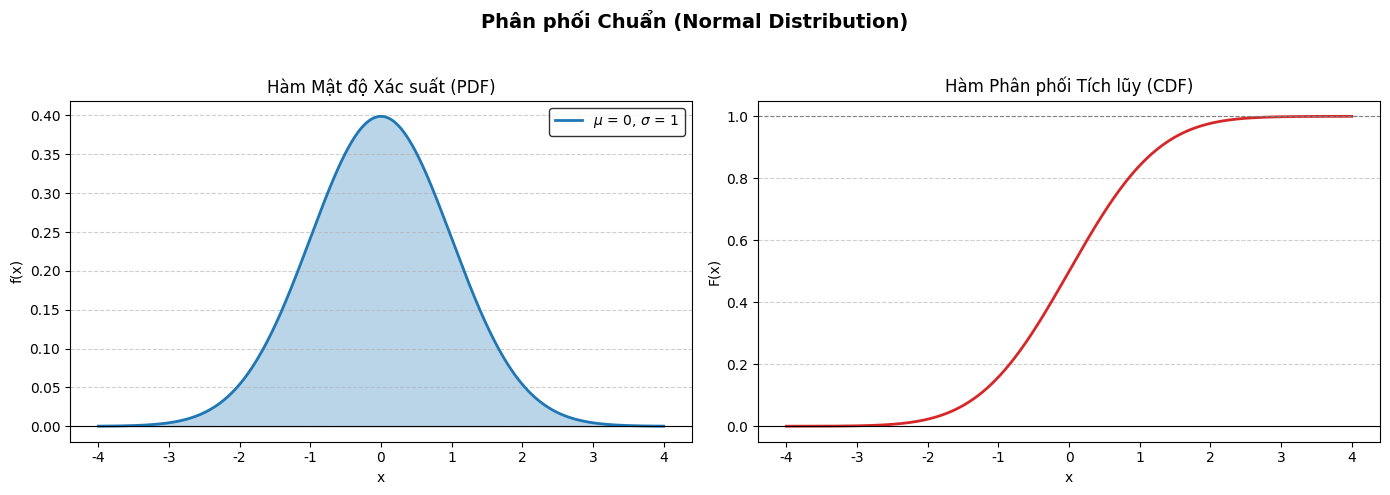
\includegraphics[width=0.8\textwidth]{images/Normal_PDF_and_CDF.png}
    \caption{Biểu đồ Hàm Mật độ Xác suất (PDF) và Hàm Phân phối Tích lũy (CDF) của Phân phối Chuẩn.}
    \label{fig:normal_dist}
\end{figure}

\subsection{Các đặc trưng thống kê}
\begin{itemize}
    \item \textbf{Kỳ vọng (Mean):} 
    \[
    \mathbb{E}[X] = \mu
    \]
    \item \textbf{Phương sai (Variance):} 
    \[
    \mathrm{Var}(X) = \sigma^2
    \]
    \item \textbf{Mode (Giá trị có xác suất cao nhất):} $\mathrm{mode} = \mu$.
    \item \textbf{Median (Trung vị):} $\mathrm{median} = \mu$.
    \item \textbf{Skewness (Độ lệch):} $\gamma_1 = 0$ (phân phối đối xứng).
    \item \textbf{Excess kurtosis (Hệ số nhọn dư):} $\gamma_2 = 0$ (kurtosis chuẩn bằng 3).
    \item \textbf{Miền xác định:} $x \in (-\infty, +\infty)$.
\end{itemize}

\subsection{Tính chất hình dạng (Shape)}

\begin{itemize}
    \item Phân phối chuẩn có \textbf{dạng đường cong hình chuông đối xứng} (\textit{bell curve}) quanh trung bình $\mu$.
    \item \textbf{Đối xứng hoàn hảo}: trung bình, trung vị và mode đều trùng tại $\mu$.
    \item \textbf{Độ lệch} (skewness) = 0; \textbf{kurtosis chuẩn} = 3 (excess kurtosis = 0).
\end{itemize}

\subsection{Ví dụ dữ liệu và ứng dụng thực tế }

\paragraph{Ứng dụng 1: Điểm thi, chiều cao, chỉ số IQ.}  
Nhiều đặc tính sinh học và xã hội (ví dụ: chiều cao của người trưởng thành trong một quần thể, điểm IQ, điểm thi chuẩn hoá) được mô tả rất tốt bởi phân phối chuẩn.  
Lý do là vì các đặc tính này chịu ảnh hưởng của nhiều yếu tố ngẫu nhiên nhỏ, độc lập (yếu tố di truyền, môi trường, rèn luyện, ...), và theo \textbf{Định lý giới hạn trung tâm}, tổng hợp của các yếu tố này sẽ xấp xỉ phân phối chuẩn.

Ví dụ, điểm IQ trong dân số thường được mô hình hoá theo phân phối:
\[
X \sim \mathcal{N}(100,\;15^2)
\]
Xác suất để một người có IQ lớn hơn 130 là:
\[
P(X > 130) = 1 - \Phi\Bigl(\frac{130 - 100}{15}\Bigr) 
= 1 - \Phi(2) \approx 0.0228,
\]
tức khoảng 2.28\% dân số.

\paragraph{Ứng dụng 2: Kiểm định giả thuyết và khoảng tin cậy.}  
Phân phối chuẩn là nền tảng cho nhiều phương pháp thống kê suy luận, đặc biệt là khi làm việc với mẫu lớn hoặc phương sai tổng thể đã biết.  


\section{Phân phối Mũ}

\subsection{Định nghĩa}

Phân phối mũ mô tả thời gian giữa các sự kiện liên tiếp trong một quá trình Poisson với tốc độ (rate) không đổi.  
Nó là phiên bản liên tục tương ứng của phân phối hình học.  

Ta ký hiệu:
\[
X \sim \mathrm{Exponential}(\lambda), \quad \lambda>0.
\]

\subsection{Probability Density Function - PDF}

Hàm mật độ xác suất của phân phối mũ được cho bởi:
\[
f(x;\lambda) = 
\begin{cases}
\lambda e^{-\lambda x}, & x \ge 0, \\
0, & x < 0.
\end{cases}
\]

\subsection{Cumulative Distribution Function - CDF}

Hàm xác suất tích lũy được định nghĩa là:
\[
F(x;\lambda) = P(X \le x) =
\begin{cases}
0, & x < 0,\\[0.5em]
1 - e^{-\lambda x}, & x \ge 0.
\end{cases}
\]

\begin{figure}[h!]
 \centering
 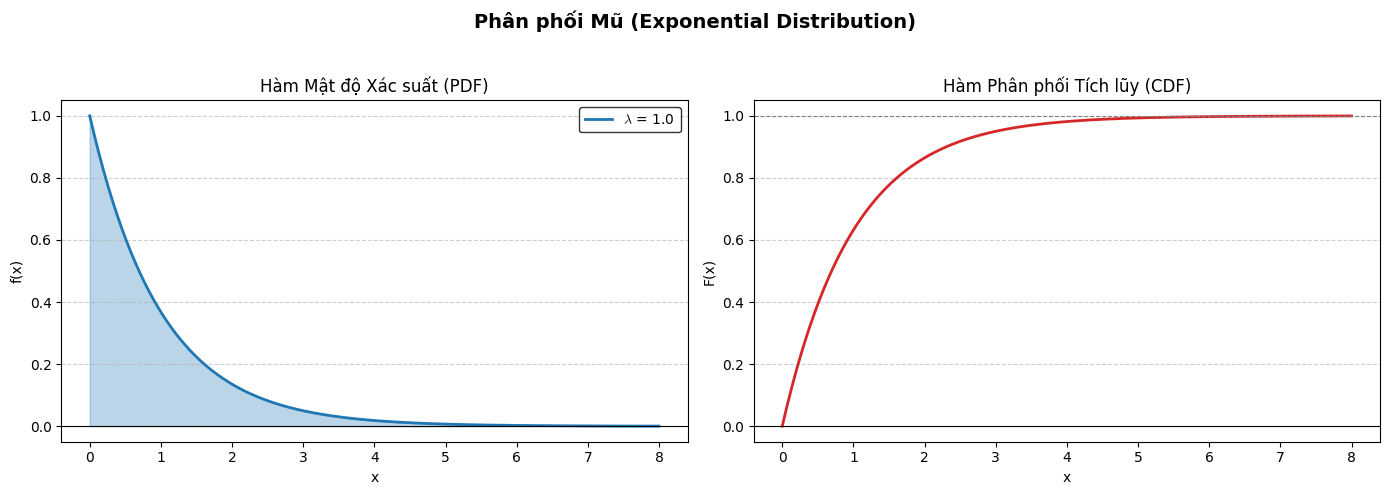
\includegraphics[width=0.8\textwidth]{images/Exp_PDF_and_CDF.png}
\caption{Biểu đồ Hàm Mật độ Xác suất (PDF) và Hàm Phân phối Tích lũy (CDF) của Phân phối Mũ.}
\label{fig:exponential_dist}
\end{figure}

\subsection{Các đặc trưng thống kê}

\begin{itemize}
    \item \textbf{Giá trị kỳ vọng (Mean):}
    \[
    \mathbb{E}[X] = \frac{1}{\lambda}
    \]
    \item \textbf{Phương sai (Variance):}
    \[
    \mathrm{Var}(X) = \frac{1}{\lambda^2}
    \]
    \item \textbf{Mode:} $0$
    \item \textbf{Median:}
    \[
    \mathrm{Median}(X) = \frac{\ln 2}{\lambda}
    \]
    \item \textbf{Miền xác định:} $x \in [0, +\infty)$
\end{itemize}

\subsection{Tính chất hình dạng (Shape)}

\begin{itemize}
    \item Phân phối mũ có \textbf{dạng hàm mật độ giảm đơn điệu} trên $[0,\infty)$, với \textbf{đỉnh tại $x=0$} và giảm theo hàm mũ khi $x$ tăng.
    \item \textbf{Lệch phải rõ rệt}: Skewness $= 2$, Kurtosis chuẩn $= 9$ (excess kurtosis $= 6$) $\Rightarrow$ đuôi phải dày hơn chuẩn.
    \item \textbf{Không đối xứng}: chỉ có một đuôi phải, giảm theo $e^{-\lambda x}$.
    \item \textbf{Tính không nhớ}: $P(X > s + t \mid X > s) = P(X > t)$, đặc trưng riêng của phân phối mũ.
\end{itemize}

\subsection{Ví dụ dữ liệu và ứng dụng thực tế}

\paragraph{Ứng dụng 1: Độ tin cậy sản phẩm và thời gian hỏng hóc.}  
Phân phối mũ thường được sử dụng để mô hình hóa \textit{thời gian giữa các hỏng hóc} của linh kiện điện tử, thiết bị cơ khí hoặc hệ thống, đặc biệt khi \textbf{tốc độ hỏng hóc không thay đổi theo thời gian}. Đây là giả định thường gặp trong giai đoạn hoạt động ổn định của sản phẩm (không tính giai đoạn “hao mòn ban đầu” hoặc “lão hóa”).

\paragraph{Ứng dụng 2: Quản lý lưu lượng và hàng đợi.}  
Trong các hệ thống xếp hàng (ví dụ: khách đến cửa hàng, gói tin đến máy chủ), thời gian giữa các lượt đến thường được giả định là phân phối mũ.

\end{document}
